\documentclass[11pt,a4paper]{article}
\usepackage[margin=2.5cm]{geometry}
\usepackage[T1]{fontenc}
\usepackage[utf8]{inputenc}
\IfFileExists{lmodern.sty}{\usepackage{lmodern}}{}
\usepackage{amsmath,amssymb,amsthm,bm}
\usepackage{booktabs,multirow,array}
\usepackage{graphicx}
\usepackage{xcolor}
\usepackage{tikz}
\usetikzlibrary{arrows.meta,positioning,shapes.geometric,fit,calc}
\usepackage{siunitx}
\usepackage{enumitem}
\usepackage{caption}
\usepackage[colorlinks=true,linkcolor=blue!50!black,citecolor=blue!50!black,urlcolor=blue!50!black]{hyperref}

\sisetup{detect-all, group-separator={,}, group-minimum-digits=4}
\captionsetup{font=small,labelfont=bf}
\setlist{nosep,leftmargin=*}

\newtheorem{definition}{Definition}
\newcommand{\R}{\mathbb{R}}
\newcommand{\rf}{r_{\mathrm{f}}}     % closed end (row)
\newcommand{\rs}{r_{\mathrm{s}}}     % channel exit (row)
\newcommand{\cost}{\mathrm{c}}
\newcommand{\ind}{\mathbf{1}}
\newcommand{\hatp}{\hat p}

\title{Automated detection, tracking and lineage reconstruction of \emph{E.~coli}\\ in mother-machine time-lapse images\\[4pt] \large Methods (working draft)}
\author{}
\date{Pipeline version of 7 November 2026\\[2pt] \small Code: \url{https://github.com/jmolina07developer/mother-machine-pipeline}}

\begin{document}
\maketitle

\begin{abstract}
\noindent
We describe the image-analysis pipeline used to quantify single-cell growth, division and survival of \emph{Escherichia coli} in a mother machine~\cite{wang2010}. Bright-field images are assembled into registered stacks, each growth channel is straightened into a one-dimensional strip, and cells are detected in every frame by a centre-based convolutional network that predicts, for every row of the strip, the probability of a cell centre, the distances to the two cell poles and a row class. Detections are linked into lineages by solving, for each channel and for the whole movie at once, an integer linear program whose variables encode which detections are cells, how cells continue, divide, appear and leave, and whose constraints enforce that every detection is explained exactly once and that cells cannot overtake each other in the channel. On held-out frames (\num{919} frames, \num{3406} manually annotated cells, four experimental conditions) the detector reaches a precision of \SI{98.5}{\percent} and a recall of \SI{96.9}{\percent} with a median pole error of \SI{0.56}{px}. Compared with lineages built from manual annotations (46 channels, \num{14454} links), the global tracker reproduces \SI{97.7}{\percent} of the frame-to-frame links and \SI{85.3}{\percent} of the division links.
\end{abstract}

\tableofcontents

%======================================================================
\section{Overview}
%======================================================================

The pipeline (Fig.~\ref{fig:overview}) takes the raw bright-field images of each microscope position and produces, for every growth channel, two tables: one row per cell and frame (position of both poles, length, flags) and one row per cell (birth, division or fate, length at birth and at division, growth rate, mother). When a fluorescence channel is present, a third table gives the background-corrected fluorescence of every cell in every frame (\S\ref{sec:fluo}). All steps run on a standard laptop CPU; a typical position (25 channels, \numrange{30}{180} frames) takes \SIrange{20}{90}{\second}.

\begin{figure}[ht]
\centering
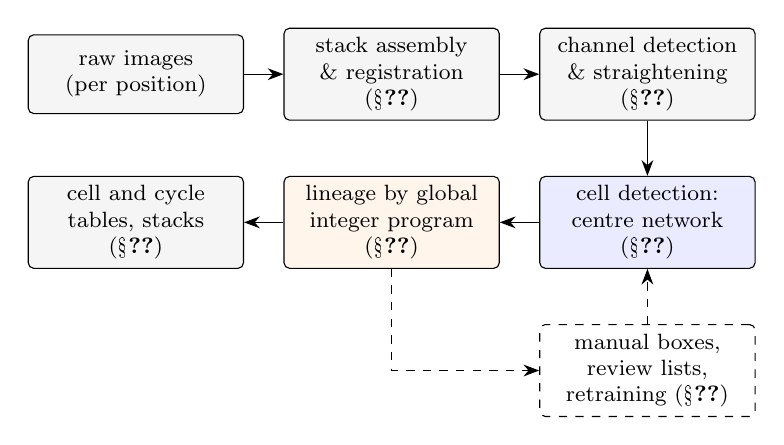
\begin{tikzpicture}[node distance=5mm and 5mm, every node/.style={font=\footnotesize},
  box/.style={draw, rounded corners=2pt, align=center, minimum height=10mm, text width=25mm, fill=#1!8},
  box/.default=gray, >={Stealth[length=2mm]}]
\node[box=gray] (raw) {raw images\\(per position)};
\node[box=gray, right=of raw] (stk) {stack assembly\\\& registration\\(\S\ref{sec:stacks})};
\node[box=gray, right=of stk] (ch) {channel detection\\\& straightening\\(\S\ref{sec:channels})};
\node[box=blue, below=7mm of ch] (det) {cell detection:\\centre network\\(\S\ref{sec:detector})};
\node[box=orange, left=of det] (trk) {lineage by global\\integer program\\(\S\ref{sec:tracking})};
\node[box=gray, left=of trk] (out) {cell and cycle\\tables, stacks\\(\S\ref{sec:outputs})};
\draw[->] (raw) -- (stk); \draw[->] (stk) -- (ch); \draw[->] (ch) -- (det); \draw[->] (det) -- (trk); \draw[->] (trk) -- (out);
\node[draw, dashed, rounded corners=2pt, align=center, text width=25mm, below=7mm of det] (ann) {manual boxes,\\review lists,\\retraining (\S\ref{sec:training})};
\draw[->, dashed] (ann) -- (det); \draw[->, dashed] (trk) |- (ann);
\end{tikzpicture}
\caption{Pipeline overview. The detector is trained on boxes drawn by hand on the straightened channels; the tracker proposes frames where the detections are doubtful, which are reviewed and added to the training set (dashed loop).}
\label{fig:overview}
\end{figure}

\paragraph{Coordinates and units.} After straightening (\S\ref{sec:channels}) a channel is a strip of $L$ rows (along the channel axis) by $W$ columns. Row $r=0$ lies \SI{10}{px} above the closed end of the channel, whose row is $\rf$ (so $\rf\approx 10$); the channel exit, where cells are washed into the main trench, is at row $\rs$. A cell in a frame is a \emph{box}, i.e.\ an interval $[a,b]$ of rows, where $a$ is the top (old or new) pole, closest to the closed end, and $b$ the bottom pole; its length is $L=b-a$. Box edges use the ImageJ~\cite{schneider2012} convention: row $r$ covers the interval $[r,r+1)$, so its centre is $r+\tfrac12$. All lengths are in pixels (the pixel size is a single multiplicative constant and does not affect any ratio, rate or test reported here); times are minutes, taken from the acquisition time stamp of every image.

%======================================================================
\section{Stack assembly and registration}\label{sec:stacks}
%======================================================================

\paragraph{Inventory.} Image files are named \texttt{<position>\_<yymmdd>\_<hhmmss>\_\ldots.tif}; the name gives the position and the acquisition time of every image. Bright-field and fluorescence images are told apart by their brightness: the median intensities of all images are split into two groups with Otsu's threshold~\cite{otsu1979}, and if the darker group is less than half as bright as the brighter one its images are fluorescence (otherwise all images are treated as bright field). When several fluorescence channels were acquired (e.g.\ GFP and propidium iodide), they are separated by multi-level Otsu thresholds~\cite{liao2001} on the logarithm of the median intensity. Each fluorescence image is paired with the bright-field image of the same position acquired within \SI{60}{\second}; a fluorescence channel need not be imaged at every time point (slices without an image are left empty and are not measured). Positions with fewer than 10 images are ignored.

\paragraph{Consistency checks.} Some acquisition errors are corrected before the stacks are built; all of them use the normalised cross-correlation (NCC) of the chip numbers defined below.
\begin{enumerate}[label=(\roman*)]
\item \emph{Shifted position numbers.} Every bright-field image is compared with a reference image (the middle of the movie) of its own position and of the two neighbouring positions. An image that matches a neighbour with $\mathrm{NCC}\ge0.85$ and at least $0.15$ better than its own position is moved there, together with its fluorescence image; if it matches neither, shifts of up to $\pm6$ positions are tried.
\item \emph{Repeated bright-field images.} When two or more bright-field images of a position are less than \SI{60}{\second} apart, only one is kept: the one with a paired fluorescence image and, among those, the one that best matches the chip numbers of its position (on a tie, the first). An unpaired bright-field image right after a paired one is also discarded if it was taken less than half a frame interval later, or if it lies between two paired images and does not match the chip numbers of its position ($\mathrm{NCC}<0.5$; an image of another field).
\item \emph{Two fields under one number.} In positions with bright field only, two near-simultaneous images whose chip numbers are displaced by more than \SI{25}{px} are two different fields of the chip saved under the same position number, and are split into two series.
\item \emph{Images discarded by hand.} Images listed in a file (e.g.\ a frame of another field of the chip saved under a position) are removed from the inventory.
\item \emph{Exposure changes.} If, for some images, the range between the 1st percentile and the median differs by more than \SI{10}{\percent} from its median over the stack (the exposure was changed during the movie), each such image is mapped linearly so that its 1st percentile and its median become the medians over the stack.
\end{enumerate}
Each bright-field stack is then converted to 8 bits by linear scaling between its \num{0.1} and \num{99.9} percentiles; fluorescence is kept at 16 bits (\S\ref{sec:fluo}).

\paragraph{Rotation.} The chip can be slightly rotated after it is repositioned (in one experiment the orientation changed in steps of $-1.2^\circ$, $-1.0^\circ$, $0^\circ$, $+0.8^\circ$ and $+1.3^\circ$ during the movie). Because the modulus of the Fourier transform is invariant to translation and rotates with the image, the rotation of each slice is the angular shift between the magnitude spectra resampled in polar coordinates, found by phase correlation~\cite{reddy1996} (difference-of-Gaussians filtered, Hann-windowed central square of the image; 3600 angular bins, upsampled phase correlation). The periodic channels give strongly oriented spectra, and the precision is $\approx0.02^\circ$. Rotations are measured relative to the median orientation of the stack; slices rotated by more than $0.1^\circ$ are rotated back by bilinear interpolation (fluorescence slices with the same angle), and measurements above $5^\circ$ are discarded as unreliable.

\paragraph{Registration.} The chip carries printed numbers above the channels that do not change in time, so every slice is registered to a reference slice using that region. Let $I_t$ be slice $t$ and $B_t = I_t * (G_{\sigma=2} - G_{\sigma=20})$ its difference-of-Gaussians band-pass filtered version~\cite{marr1980} (it keeps the edges of the digits and removes illumination gradients), restricted to rows $0$--$450$. The template $T$ is the reference $B_{\mathrm{ref}}$ with a margin of $m=\SI{80}{px}$ removed on every side, and the displacement of slice $t$ is the maximiser of the normalised cross-correlation~\cite{lewis1995}, computed with \texttt{match\_template} of scikit-image~\cite{vanderwalt2014}
\begin{equation}
\mathrm{NCC}_t(\Delta y,\Delta x)=\frac{\sum_{i,j}\bigl(B_t(i+\Delta y,j+\Delta x)-\bar B_t\bigr)\bigl(T(i,j)-\bar T\bigr)}{\sqrt{\sum_{i,j}\bigl(B_t(i+\Delta y,j+\Delta x)-\bar B_t\bigr)^2\;\sum_{i,j}\bigl(T(i,j)-\bar T\bigr)^2}},\qquad |\Delta y|,|\Delta x|\le m,
\end{equation}
where $\bar B_t$ is the mean of the window under the template. The maximum value is reported as the registration quality (1 = perfect match). The reference is chosen among the slices at \SIlist{0;25;50;75}{\percent} of the movie as the one with the highest median quality against a sample of 12 slices; slices with quality $<0.8$ are re-registered through the other candidate references (composing the two displacements). Slices whose quality is still below $0.93$ are searched again over all displacements of up to \SI{500}{px} with a masked normalised cross-correlation computed in the Fourier domain~\cite{padfield2012} (overlap of at least \SI{35}{\percent} of the image; at half resolution, then refined by $\pm\SI{2}{px}$), and the new displacement is kept if it raises the quality by more than $0.02$ and reaches at least $0.8$ (with blurred images the unrestricted search can otherwise lock onto a spurious match). This recovers stage jumps of several hundred pixels, for which the restricted search locks onto a neighbouring block of the chip numbers, which repeat every $\approx\SI{200}{px}$ (quality $\approx0.7$--$0.86$ instead of $>0.95$). After such a jump part of the registered slice has no image (it is filled with the median grey); every channel--frame whose central half (\S\ref{sec:channels}) falls outside the real image is treated as a bad frame of that channel by the tracker and is not used for training. Slices are shifted by an integer number of pixels (no interpolation beyond the rotation above). When the stage drifts by more than the margin (e.g.\ $>\SI{200}{px}$ vertically), the search region can be extended to the whole image, so that the bottom edge of the channel array also contributes, together with a larger margin ($m=\SI{160}{px}$). As an independent check, each registered slice is matched against the previous one with a $\pm\SI{15}{px}$ search; the residual displacement should be $0$--$\SI{1}{px}$, and larger residuals are reported (``doubtful alignment'').

%======================================================================
\section{Channel detection and straightening}\label{sec:channels}
%======================================================================

Channels are found on the temporal mean $\bar I$ of the registered stack. Rows that belong to the channel band are those whose intensity profile is periodic (normalised autocorrelation $>0.4$ at a lag between \num{20} and \SI{80}{px}) and that contain strong vertical edges (the channel walls). In the band, the column profile is smoothed with a Gaussian of width $P/7$ ($P$ = period of the comb, from the autocorrelation) and its local minima, i.e.\ the dark channel interiors, give the channel centres; channels cut by the image border are added if the comb continues and the local contrast is similar to the other channels. For each channel, the centre is measured at several heights and a line $x=\beta_0+\beta_1 y$ is fitted by least squares (the channel axis); the closed end and the exit are the extremes of the region where wall edges are present along that axis.

Each channel is straightened by bilinear interpolation along its axis (\texttt{map\_\allowbreak coordinates} of SciPy~\cite{virtanen2020}): with $\mathbf p_0$ the closed-end point, $\mathbf u$ the unit vector along the axis and $\mathbf n\perp\mathbf u$,
\begin{equation}
S_t(r,w)=I_t\!\left(\mathbf p_0+(r-10)\,\mathbf u+\bigl(w-\tfrac{W-1}{2}\bigr)\mathbf n\right),\qquad r=0,\dots,L-1,\;\; w=0,\dots,W-1,
\end{equation}
with $W$ the largest odd integer not above $0.8P$ (so that the walls are visible). The strips of all frames of a channel are placed side by side in one image (one image per channel), which is the image used both for manual annotation and for detection. The same sampling gives the kymograph of each channel (intensity along the axis versus time).

%======================================================================
\section{Cell detection with a centre-based network}\label{sec:detector}
%======================================================================

\subsection{Formulation}
In a straightened channel, cells are stacked along the rows and touch each other, so detection is a one-dimensional problem: find the set of intervals $\{[a_i,b_i]\}$ occupied by cells in each frame. Instead of segmenting pixels, the network represents every cell by its centre $c_i=(a_i+b_i)/2$, in the spirit of CenterNet~\cite{zhou2019}: two touching cells have distinct centres even when the septum between them is faint, so they are not merged. For each row $r$ the network outputs
\begin{itemize}
\item $\hatp_r\in(0,1)$, the probability that a cell centre lies in row $r$ (centre map);
\item $\hat d^{\,\mathrm{top}}_r,\hat d^{\,\mathrm{bot}}_r>0$, the distances from the row centre $r+\tfrac12$ to the top and bottom pole of that cell;
\item $\hat q_{r,k}$, $k\in\{0,1,2,3\}$, the probabilities that row $r$ is background, cell interior, top pole or bottom pole (row classes, $\sum_k\hat q_{r,k}=1$).
\end{itemize}
Figure~\ref{fig:maps} shows the three outputs for one test frame.

\begin{figure}[ht]
\centering
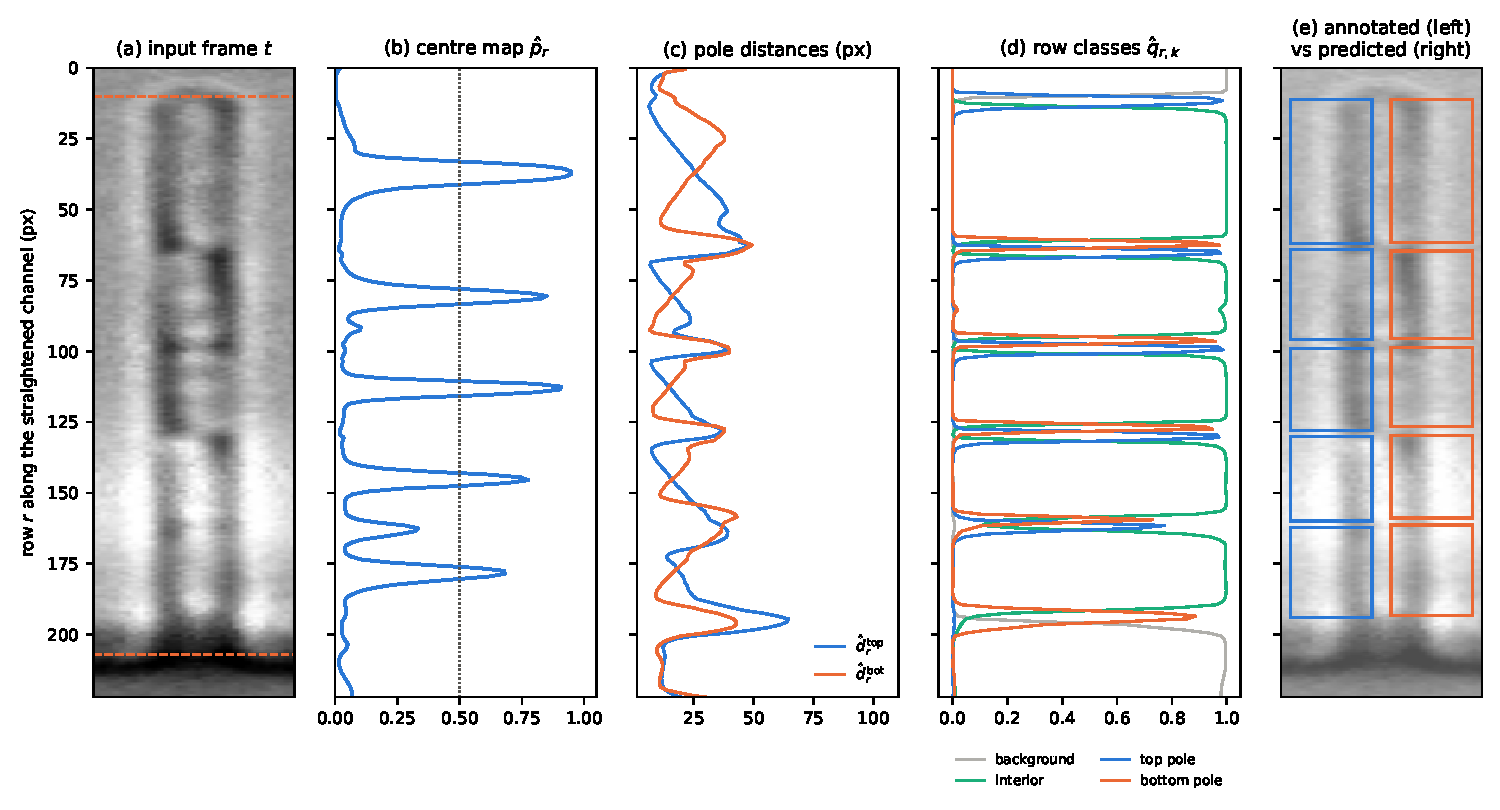
\includegraphics[width=\textwidth]{fig/detector_maps.pdf}
\caption{Detector outputs for one held-out frame (LB, position 04, channel 5, frame 59). (a)~Straightened channel; dashed lines: closed end $\rf$ and exit $\rs$. (b)~Centre map with the threshold $0.5$ (dotted). (c)~Predicted distances to the two poles. (d)~Row-class probabilities. (e)~Manually annotated boxes (left half) and decoded boxes (right half).}
\label{fig:maps}
\end{figure}

\subsection{Input}
The network sees frame $t$ together with its neighbours $t-2,\dots,t+2$ (indices clamped to the movie), because what moves between frames is a cell and what stays still is dirt or chip structure. Each strip is cropped or zero-padded to a fixed size of $L_0\times W_0=288\times 32$ (centred across the width, padded below), and each of the five frames $u$ is standardised over its non-zero (non-padding) pixels,
\begin{equation}
X_u(r,w)=\frac{S_u(r,w)-m_u}{\max(s_u,1)},\qquad m_u=\operatorname{mean}\{S_u>0\},\;\; s_u=\operatorname{sd}\{S_u>0\},
\end{equation}
where the floor $\max(s_u,1)$ protects against blank or saturated frames. Two more input planes encode the position along the channel, $(r-\rf)/100$ and $(r-\rs)/100$, constant across the width. The input tensor therefore has $C_{\mathrm{in}}=5+2=7$ planes of $288\times 32$.

\subsection{Architecture}
The network (\num{745463} parameters; Table~\ref{tab:arch}) first summarises the width of the channel with 2D convolutions and then works along the channel axis with a 1D U-Net~\cite{ronneberger2015}. Blocks are two convolutions (kernel 3), each followed by batch normalisation~\cite{ioffe2015} and a rectified linear unit (ReLU)~\cite{nair2010}. A $1\times 8$ convolution collapses the remaining 8 columns, leaving a sequence of length 288 with 64 features. The 1D U-Net has three down-sampling levels (max-pooling by 2), the deepest with dilated convolutions~\cite{yu2016} (dilation 2 and 4) to see whole long cells, and three up-sampling levels (nearest-neighbour interpolation followed by concatenation with the skip connection of the same level). Three $1\times1$ convolutions produce the outputs: the centre logit $z_r$ with $\hatp_r=\operatorname{sigmoid}(z_r)$ (bias initialised to $-2.2$, i.e.\ $\hatp\approx0.1$, as centres are rare), the distances $\hat d=10\,\operatorname{softplus}(\cdot)$, and four class logits followed by a softmax.

\begin{table}[ht]
\centering\small
\caption{Network layers. $B$: batch, $C$: features, shapes are (features, rows, columns).}
\label{tab:arch}
\resizebox{\textwidth}{!}{%
\begin{tabular}{@{}lll@{}}
\toprule
Stage & Operation & Output shape\\
\midrule
input & 5 standardised frames + 2 position planes & $7\times288\times32$\\
2D encoder & block(16), max-pool $1\times2$ & $16\times288\times16$\\
 & block(32), max-pool $1\times2$ & $32\times288\times8$\\
 & block(64), conv $1\times8$ + BN + ReLU & $64\times288$\\
1D U-Net & block(64) & $64\times288$\\
 & pool, block(96); pool, block(128); pool, block(128, dil.~2) + block(128, dil.~4) & $96{\times}144$, $128{\times}72$, $128{\times}36$\\
 & up + skip, block(128); up + skip, block(96); up + skip, block(64) & $64\times288$\\
heads & conv $1{\times}1$: centre (1), distances (2), classes (4) & $1,2,4\times288$\\
\bottomrule
\end{tabular}}
\end{table}

\subsection{Training targets}
For a frame with manually annotated boxes $\{[a_i,b_i]\}$, with centre $c_i$ and length $n_i=b_i-a_i$, the targets are defined row by row ($\rho=r+\tfrac12$ is the centre of row $r$).

\emph{Centre map.} A Gaussian bump per cell, with width proportional to its length,
\begin{equation}
Y_r=\max_i \exp\!\left(-\frac{(\rho-c_i)^2}{2s_i^2}\right),\qquad s_i=\max(1.5,\,n_i/6),
\end{equation}
and $Y_r=1$ exactly at the row that contains $c_i$ (the positive row of cell $i$).

\emph{Pole distances.} For the rows near the centre, $|\rho-c_i|\le\max(1,n_i/4)$, the targets are $d^{\mathrm{top}}_r=\rho-a_i$ and $d^{\mathrm{bot}}_r=b_i-\rho$, and the mask is $M_r=1$; elsewhere $M_r=0$.

\emph{Row classes.} $y_r=1$ (interior) inside a box, $y_r=2$ for the three rows around each top pole and $y_r=3$ for the three rows around each bottom pole, $y_r=0$ (background) elsewhere. Rows more than 3 px below the lowest annotated box are not annotated (the annotator only draws cells that can be identified with certainty); they count as background with weight $w_r=0.5$. Rows of boxes proposed by the detector and \emph{deleted} by the annotator are background with weight $w_r=3$ (they are explicit negatives); all other rows have $w_r=1$.

\subsection{Loss}
With $p_r=\hatp_r$ clipped to $[10^{-4},1-10^{-4}]$ and $N_+=\#\{r:Y_r=1\}$,
\begin{align}
\mathcal L_{\mathrm{centre}}&=-\frac{1}{N_+}\sum_r w_r\Bigl[\ind_{Y_r=1}\,(1-p_r)^2\log p_r+\ind_{Y_r<1}\,(1-Y_r)^4\,p_r^2\log(1-p_r)\Bigr],\label{eq:focal}\\
\mathcal L_{\mathrm{dist}}&=\frac{1}{2\sum_r M_r}\sum_r M_r\sum_{e\in\{\mathrm{top},\mathrm{bot}\}}\bigl|\log(1+\hat d^{\,e}_r)-\log(1+d^{\,e}_r)\bigr|,\\
\mathcal L_{\mathrm{class}}&=\frac{\sum_r w_r\,\pi_{y_r}\,\bigl(-\log\hat q_{r,y_r}\bigr)}{\sum_r w_r},\qquad \pi_k=\sqrt{\frac{N}{4N_k}},\\
\mathcal L&=\mathcal L_{\mathrm{centre}}+\mathcal L_{\mathrm{dist}}+\tfrac12\,\mathcal L_{\mathrm{class}}.
\end{align}
Eq.~\eqref{eq:focal} is the penalty-reduced focal loss of CenterNet~\cite{lin2017,zhou2019}: the factor $(1-p)^2$ focuses learning on the hard positives, $p^2$ on the hard negatives, and $(1-Y_r)^4$ reduces the penalty for predicting a centre close to a true one. The distance loss is an $L_1$ loss on $\log(1+d)$, so that a 1-px error matters more for a short cell than for a long filament. In the class loss, $N_k$ is the (weighted) number of training rows of class $k$ and $N=\sum_kN_k$; the weights $\pi_k$ compensate for poles being much rarer than background and interior rows.

\subsection{Training data and procedure}\label{sec:training}
\paragraph{Annotation.} Cells are annotated as boxes on the straightened channels with a macro for Fiji~\cite{schindelin2012}: the annotator corrects boxes proposed by the current detector (adds missing cells, moves edges, deletes wrong boxes) and marks bad frames (out of focus, wrong field, flow artefacts), which are excluded. Frames are proposed for review in two ways: (i)~frames where the detector is uncertain (a box with confidence below $0.6$), and (ii)~frames where the tracker of \S\ref{sec:tracking} has doubts. For (ii) every frame of every channel is scored by the tracker's solution: a cell that the network missed but the tracker knows was there (weight 3), a cell split in two by the network (3), a detection rejected as a false positive (2), a cell that disappears inside the channel (2; not in frames 1--3, when cells are flushed while the chip is loaded), a box whose length does not match the expected one (1) and a division (1). In each image the $n$ highest-scoring frames (at most two per channel, at least 4 frames apart) are proposed, plus \SI{15}{\percent} random frames so that the training set does not contain only difficult cases.

\paragraph{Data set.} The installed model was trained on \num{6391} annotated channel-frames from 297 channels of 20 images (LB; ciprofloxacin; gentamicin $\to$ ciprofloxacin sequences; ciprofloxacin $\to$ gentamicin), split \emph{by channel}: \num{5076} frames for training, 468 frames (24 channels, $\approx\SI{10}{\percent}$) for validation, i.e.\ for choosing the epoch and the centre threshold, and a fixed test set of 847 frames (later extended to 919) from channels that are never used for training. Whenever new annotations were added, \SI{30}{\percent} of the channels containing new frames were moved to the test set.

\paragraph{Optimisation.} The network is implemented and trained in PyTorch~\cite{paszke2019}. AdamW~\cite{loshchilov2019} (weight decay $10^{-4}$), one-cycle learning-rate schedule~\cite{smith2019} with maximum $2\times10^{-3}$ and \SI{10}{\percent} warm-up, batch size 16, 14 epochs; the checkpoint with the highest validation F1 is kept. Data augmentation, applied to the five image planes: a random gain $\sim U(0.8,1.25)$ and offset $\sim\mathcal N(0,0.15^2)$, pixel noise $\sim\mathcal N(0,0.05^2)$, with probability $0.15$ the four neighbours are replaced by frame $t$ itself (as at the start or end of a movie), and with probability $0.5$ a left--right flip. Training takes $\approx\SI{30}{\minute}$ on two CPU cores. For inference the network is exported to ONNX~\cite{onnx} and run with ONNX Runtime~\cite{onnxruntime}, so the pipeline does not need PyTorch.

\subsection{From maps to boxes}\label{sec:decode}
\begin{enumerate}
\item \emph{Peaks.} Candidate centres are the rows $r$ with $\hatp_r\ge0.5$ that are local maxima within $\pm3$ rows. The value $\hatp_r$ at the peak is the confidence of the box.
\item \emph{Edges.} The poles are averaged over the three rows around the peak with weights $\hatp$:
\begin{equation}
a=\frac{\sum_{r'=r-1}^{r+1}\hatp_{r'}\,(r'+\tfrac12-\hat d^{\,\mathrm{top}}_{r'})}{\sum_{r'}\hatp_{r'}},\qquad
b=\frac{\sum_{r'=r-1}^{r+1}\hatp_{r'}\,(r'+\tfrac12+\hat d^{\,\mathrm{bot}}_{r'})}{\sum_{r'}\hatp_{r'}};
\end{equation}
boxes shorter than \SI{5}{px} are discarded.
\item \emph{Non-maximum suppression in 1D.} Boxes are visited in decreasing confidence and a box is dropped if it overlaps an already kept box by more than half the length of the shorter one.
\item \emph{Sub-pixel pole refinement.} The top pole is moved to the maximum of the top-pole probability $\hat q_{\cdot,2}$ within $\pm3$ rows of $a$, refined by fitting a parabola through the maximum row $k$ and its two neighbours:
\begin{equation}
k^\star=k+\frac{1}{2}\,\frac{\hat q_{k-1}-\hat q_{k+1}}{\hat q_{k-1}-2\hat q_k+\hat q_{k+1}},\qquad a\leftarrow k^\star-\tfrac12,
\end{equation}
if that maximum probability is at least $0.2$ (and likewise the bottom pole with $\hat q_{\cdot,3}$ and $b\leftarrow k^\star+\tfrac12$).
\item Remaining small overlaps between consecutive boxes are split at the midpoint.
\end{enumerate}

\subsection{Evaluation of the detector}\label{sec:det_eval}
In every test frame the predicted boxes are compared with the annotated ones inside the annotated zone (above the lowest annotated box plus 3 px). Predicted and true boxes are matched one-to-one by maximising the total intersection over union (IoU, Hungarian algorithm~\cite{kuhn1955}, as implemented in \texttt{scipy.optimize.\allowbreak linear\_\allowbreak sum\_\allowbreak assignment}~\cite{crouse2016,virtanen2020}); a match counts if $\mathrm{IoU}\ge0.5$. We report precision $=\#\text{matches}/\#\text{predicted}$, recall $=\#\text{matches}/\#\text{annotated}$, \emph{invented} boxes (predicted boxes covered less than \SI{30}{\percent} by annotated cells, inside the annotated zone or on a deleted proposal, per 100 frames), \emph{merged} boxes (one prediction containing more than \SI{60}{\percent} of each of two or more annotated cells), \emph{split} cells (one annotated cell containing more than \SI{60}{\percent} of each of two or more predictions) and the absolute error of the matched poles.

\begin{table}[ht]
\centering\small
\caption{Detector performance on held-out frames (installed model). Subsets: test channels fixed before training (``original''), frames reserved on 15/10 and on 16/10 (new positions, never used for training). Ily: images at \SI{15}{\minute} intervals and lower contrast, not represented in the training set.}
\label{tab:det}
\resizebox{\textwidth}{!}{%
\begin{tabular}{@{}lrrrrrrrr@{}}
\toprule
 & frames & cells & precision & recall & invented & merged & split & pole error (px)\\
 & & & & & /100 frames & & & median / P90\\
\midrule
All held-out frames & 919 & 3406 & 0.985 & 0.969 & 0.87 & 28 & 21 & 0.56 / 2.03\\
\addlinespace
\multicolumn{9}{@{}l}{\emph{by subset}}\\
\quad original test channels & 629 & 2172 & 0.984 & 0.975 & 0.79 & 15 & 14 & 0.53 / 2.38\\
\quad reserved 15/10 & 218 & 916 & 0.987 & 0.971 & 0.46 & 6 & 7 & 0.59 / 1.58\\
\quad reserved 16/10 (excl.\ Ily) & 53 & 268 & 0.996 & 0.933 & 0.00 & 7 & 0 & 0.66 / 1.36\\
\quad reserved 16/10, Ily & 19 & 50 & 0.957 & 0.880 & 10.5 & 0 & 0 & 0.64 / 1.22\\
\addlinespace
\multicolumn{9}{@{}l}{\emph{by condition}}\\
\quad LB (25/09) & 219 & 799 & 0.976 & 0.983 & 0.46 & 5 & 12 & 0.51 / 1.57\\
\quad CIP / GEN sequences (02/10) & 234 & 940 & 0.992 & 0.948 & 2.14 & 12 & 0 & 0.70 / 2.42\\
\quad GEN $\to$ CIP $\to$ LB (09/10) & 447 & 1617 & 0.987 & 0.977 & 0.00 & 11 & 9 & 0.55 / 1.96\\
\quad Ily (13/10) & 19 & 50 & 0.957 & 0.880 & 10.5 & 0 & 0 & 0.64 / 1.22\\
\bottomrule
\end{tabular}}
\end{table}

\paragraph{Results.} Table~\ref{tab:det} summarises the installed model. The confidence of a box is well calibrated (Table~\ref{tab:calib}): \SI{99.8}{\percent} of boxes with confidence $\ge0.9$ are correct, against $\approx\SI{84}{\percent}$ below $0.7$; boxes below $0.6$ are flagged for review.

\begin{table}[ht]
\centering\small
\caption{Calibration of the box confidence on the held-out frames: fraction of predicted boxes (inside the annotated zone) matched to an annotated cell.}
\label{tab:calib}
\begin{tabular}{@{}lrrrrr@{}}
\toprule
confidence & $[0.5,0.6)$ & $[0.6,0.7)$ & $[0.7,0.8)$ & $[0.8,0.9)$ & $[0.9,1]$\\
\midrule
boxes & 74 & 90 & 266 & 938 & 1981\\
correct & 0.838 & 0.833 & 0.966 & 0.989 & 0.998\\
\bottomrule
\end{tabular}
\end{table}

\paragraph{Development history.} The centre network replaced an earlier pixel classifier (gradient-boosted trees~\cite{friedman2001} on hand-crafted features, histogram-based as in LightGBM~\cite{ke2017}, implemented with scikit-learn~\cite{pedregosa2011}, followed by dynamic programming). It is still shipped as a fallback when ONNX Runtime is not installed. On the original 629 test frames the trees reached precision $0.956$, recall $0.958$, 4.6 invented boxes per 100 frames, 31 merged and 45 split cells, against $0.985$, $0.970$, $0.48$, 14 and 17 for the first centre network. One round of review guided by the tracker (472 new channel-frames, 15/10) raised the recall on the difficult reserved frames from \SI{93.5}{} to \SI{97.7}{\percent} (precision \SI{98.8}{} $\to$ \SI{98.5}{\percent}, median pole error $0.68\to\SI{0.60}{px}$). A second round (183 channel-frames, 16/10) did not improve the model further: networks retrained from scratch, with or without the low-quality Ily images, and networks fine-tuned from the installed one all fell within about one percentage point of it on every test subset, which is the size of the variation between training runs. The installed model was therefore kept, and the new annotations were added to the test set and to the training pool.

%======================================================================
\section{Lineage reconstruction by global integer programming}\label{sec:tracking}
%======================================================================

\subsection{Why a global formulation}
Cells in a mother-machine channel form a single file: they grow, push the cells below them towards the exit, divide into two daughters, leave through the exit, and occasionally die, lyse or are flushed out. They never overtake each other. A frame-by-frame tracker that assigns the boxes of frame $k$ to those of frame $k+1$ has to decide on the spot whether a short box is a newborn daughter, a fragment of a missed cell or a false detection. Many of these decisions can only be made by looking at several frames: a cell missed by the detector in one frame reappears in the next one; a division is confirmed by the growth of both daughters. We therefore formulate the reconstruction of a whole channel movie as a single optimisation problem: choose, among all candidate interpretations of the detections, the one with the lowest total cost, subject to consistency constraints. Because divisions turn one cell into two, this is not a plain min-cost-flow problem (as used for cell tracking in~\cite{padfield2011}), and we solve it as an integer linear program (ILP). The formulation follows the ``tracking by assignment'' family of methods~\cite{jug2014,schiegg2013}, with costs adapted to the geometry and growth of cells in a channel.

\subsection{Notation}
The movie of a channel is split into \emph{segments} of consecutive valid frames: bad frames are removed, and a new segment starts after a gap longer than $\max(\SI{20}{\minute},\,3\,\overline{\Delta t})$, where $\overline{\Delta t}$ is the median frame interval. Each segment is solved independently. Within a segment, frames are indexed $k=0,\dots,K-1$ with acquisition times $t_k$.

\begin{itemize}
\item $\mathcal D_k$: detections of frame $k$, each $j\in\mathcal D_k$ an interval $[a_j,b_j]$ with confidence $c_j\in[0.5,1]$, sorted by $a_j$. Detections starting below the exit ($a_j\ge\rs-1$) are discarded and tops are clipped at the closed end, $a_j\leftarrow\max(a_j,\rf-1)$.
\item $\mathcal N_k$: candidate \emph{nodes} (possible cells) of frame $k$: every detection, plus the union $[a_j,b_{j'}]$ of every pair of consecutive detections $j,j'$ that touch ($a_{j'}-b_j\le\kappa=\SI{4}{px}$), which covers the case of one cell split in two by the detector. Node $n$ has frame $k(n)$, interval $[a_n,b_n]$, length $L_n=b_n-a_n$ and the set $\mathcal C(n)\subseteq\mathcal D_{k(n)}$ of detections it is made of. $\mathcal N=\bigcup_k\mathcal N_k$.
\item $\ell_0$: typical newborn length, the 25th percentile of the lengths of all detections of the channel that do not touch the exit (default \SI{20}{px}).
\item $\mu(t)$: expected exponential growth rate of the position at time $t$ (\si{\per\minute}). It is estimated before tracking from all channels of the position: in each channel's kymograph cell edges are followed in time, and the relative increase of their distance to the closed end between consecutive frames, divided by the actual time interval, is a local growth rate; $\mu$ is the median over channels, smoothed with a running median of 5 frames. It follows changes of medium (e.g.\ the growth arrest under antibiotics).
\end{itemize}

\subsection{Kinematic model of a channel}
\paragraph{Growth.} A cell of length $L_n$ and growth rate $\alpha_n$ is expected, after a time $\Delta t$, to have length
\begin{equation}
\hat L_n(\Delta t)=L_n\,e^{\alpha_n\Delta t}.
\end{equation}
In the first pass $\alpha_n=\mu(t_{k(n)})$; in the second pass every cell gets its own rate (\S\ref{sec:passes}).

\paragraph{Pushing.} A cell moves down because the cells above it grow, but only those that touch it in a chain. Let $\mathcal P(n)$ be the maximal set of detections in frame $k(n)$ that lie above $n$ and form a contiguous chain down to it (consecutive gaps $\le\kappa$). The expected downward displacement of the top pole of $n$ is the growth of that chain,
\begin{equation}
s_n(\Delta t)=\sum_{i\in\mathcal P(n)}L_i\bigl(e^{\alpha_i\Delta t}-1\bigr).
\end{equation}
A cell below a gap is not pushed until the cells above reach it. The chain is \emph{free} ($\phi_n=1$) when its top cell does not sit at the closed end ($a>\rf+6$); free cells can also be moved by the flow, so their position is more uncertain.

\paragraph{Collective upward motion.} Occasionally the whole content of a channel slides towards the closed end between two frames (observed when the medium starts flowing). For each pair of consecutive frames $k,k+1$ a shift $\delta_k\le0$ is estimated. Let $a^{(k)}_1<a^{(k)}_2<\dots$ be the tops of the detections of frame $k$, $\Delta=a^{(k+1)}_1-a^{(k)}_1$ and $q=\min(3,|\mathcal D_k|-1,|\mathcal D_{k+1}|-1)\ge2$. Four hypotheses are scored by the mismatch of the first $q$ tops (each term capped at \SI{10}{px}):
\begin{align*}
C_{\text{shift}}&=\textstyle\sum_{i\le q}\bigl|(a^{(k+1)}_i-a^{(k+1)}_1)-(a^{(k)}_i-a^{(k)}_1)\bigr| && \text{(everything moved by $\Delta$)},\\
C_{\text{still}}&=\textstyle\sum_{i\le q}\bigl|a^{(k+1)}_i-a^{(k)}_i\bigr| && \text{(nothing moved)},\\
C_{\text{new top}}&=\textstyle\sum_{i\le q}\bigl|a^{(k+1)}_{i+1}-a^{(k)}_i\bigr| && \text{(nothing moved, a new box above)},\\
C_{\text{lost top}}&=\textstyle\sum_{i\le q}\bigl|a^{(k+1)}_i-a^{(k)}_{i+1}\bigr| && \text{(nothing moved, the top box was lost)}.
\end{align*}
We set $\delta_k=\Delta$ if (i) there was already a gap of at least \SI{4}{px} above the first cell in frames $k-1$ and $k$, (ii) $\SI{-40}{px}\le\Delta\le\SI{-4}{px}$, and (iii) $C_{\text{shift}}+4q\le\min(C_{\text{still}},C_{\text{new top}},C_{\text{lost top}})$; otherwise $\delta_k=0$. Between frames $k$ and $k'$ the accumulated shift is $\delta_{k\to k'}=\max\bigl(\sum_{i=k}^{k'-1}\delta_i,\;\rf-1-a_n\bigr)$ (cells cannot move above the closed end). Condition~(i) avoids confusing a collective shift with the detector missing the top cell. In the validation data the shift was triggered in 6 channels of one position (Ily 01), in no LB channel and in 0--9 channels per antibiotic position; in Ily 01 channel 13 it prevents a swap of all identities (Fig.~\ref{fig:shift}).

\paragraph{Prediction.} Combining the three effects, the expected top pole of $n$ in frame $k'$ is
\begin{equation}
\hat a_{n\to k'}=a_n+s_n(t_{k'}-t_{k(n)})+\delta_{k(n)\to k'},
\end{equation}
with positional uncertainty
\begin{equation}
\sigma_{n}=\sigma_0+\sigma_1\,|s_n|+\sigma_{\mathrm{free}}\,\phi_n\;\bigl(+\,\sigma_{\mathrm{down}}\ \text{if the observed top is below } \hat a\bigr),
\end{equation}
which grows with the predicted displacement; the extra term $\sigma_{\mathrm{down}}$ makes moving further down than predicted cheaper than moving up, because a cell can be dragged down by the flow but not pushed up. The uncertainty of a log-length is
\begin{equation}
\sigma_L(\hat L)=\sqrt{\sigma_{\log L}^2+\bigl(\sigma_{\mathrm{px}}/\hat L\bigr)^2},
\end{equation}
a relative error plus an absolute error of $\sigma_{\mathrm{px}}$ pixels (dominant for short cells).

\begin{figure}[ht]
\centering
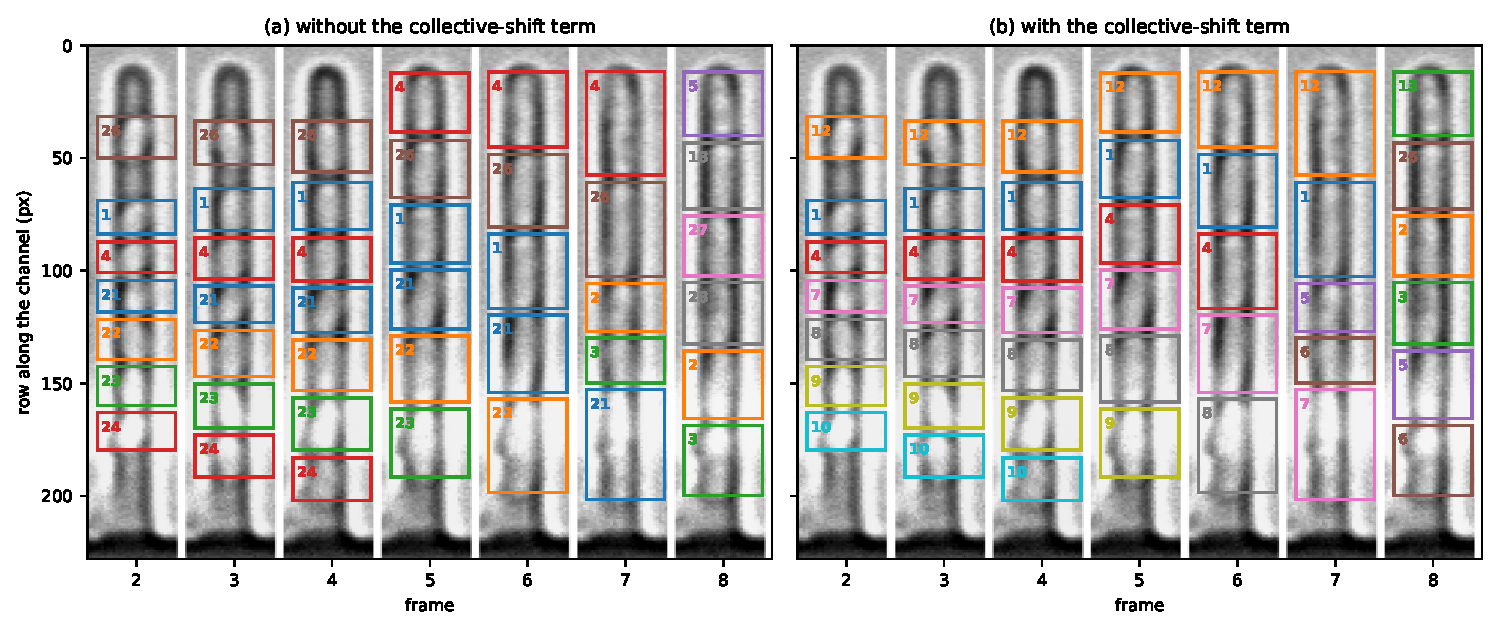
\includegraphics[width=\textwidth]{fig/collective_shift.pdf}
\caption{Effect of the collective-shift term (Ily 13/10, position 01, channel 13). Between frames 4 and 5 all cells move up by $\approx\SI{21}{px}$. (a)~Without the term, moving up is penalised, so the solver shifts every identity by one cell (the top cell is relabelled at frame 5). (b)~With $\delta_4=\SI{-21}{px}$, every cell keeps its number. Numbers are cell identifiers; colours repeat.}
\label{fig:shift}
\end{figure}

\subsection{Events and their costs}\label{sec:costs}
Costs are negative log-likelihoods up to constants, built from a robust quadratic
\begin{equation}
\rho_\tau(x)=\min\!\left(\tfrac12x^2,\;\tau\right),
\end{equation}
which behaves like a Gaussian error near zero but caps the penalty of a single gross outlier at $\tau$. All parameter values are listed in Table~\ref{tab:params}.

\paragraph{Continuation (follow) $n\to m$.} Node $n$ in frame $k$ continues as node $m$ in frame $k'=k+1+g$, where $g\in\{0,1,2\}$ is the number of frames in which the cell was not detected. With $\Delta t=t_{k'}-t_k$, $\hat a=\hat a_{n\to k'}$ and $\hat L=\hat L_n(\Delta t)$,
\begin{equation}
\cost_{n\to m}=\rho_{6}\!\left(\frac{a_m-\hat a}{\sigma_n}\right)+\rho_{12}\bigl(z^L_{nm}\bigr)+g\,\cost_{\mathrm{miss}},\qquad z^L_{nm}=\frac{\ln(L_m/\hat L)}{\sigma_L(\hat L)}.
\end{equation}
If $m$ touches the exit ($b_m\ge\rs-1.5$) its visible length is truncated, so only a length longer than expected is penalised: $z^L_{nm}\leftarrow\max(z^L_{nm},0)$. Because the costs are capped, physically impossible moves are removed explicitly (\emph{gates}): a link is not created if the top moves more than $80(1+g)$~px below $\hat a$ or above $a_n+\delta$, or more than $25(1+g)$~px above $a_n+\delta$ while passing over other detections of frame $k$ (a single cell in an almost empty channel can float up further).

\paragraph{Division $n\to(m_1,m_2)$.} Node $n$ in frame $k$ divides into an upper daughter $m_1$ and a lower daughter $m_2$, both in frame $k+1$, or one in $k+1$ and the other in $k+2$ (a daughter missed for one frame; a ``delayed'' division). Requirements: $m_2$ below $m_1$ ($a_{m_2}\ge b_{m_1}-2$), disjoint detections ($\mathcal C(m_1)\cap\mathcal C(m_2)=\emptyset$), at most \SI{6}{px} between them when simultaneous, and $|a_{m_1}-\hat a|\le\SI{40}{px}$. With the partition ratio $\pi=L_{m_1}/(L_{m_1}+L_{m_2})$ and the daughters' combined extent $S=b_{m_2}-a_{m_1}$ (or $L_{m_1}+L_{m_2}$ if delayed),
\begin{multline}
\cost_{n\to(m_1,m_2)}=\cost_{\mathrm{div}}+\rho_6\!\left(\frac{a_{m_1}-\hat a}{\sigma_n}\right)+\ind[b_{m_2}<\rs-1.5]\;\rho_4\!\left(\frac{\pi-\frac12}{\sigma_\pi}\right)\\
+\rho_{12}\!\left(\frac{\ln(S/\hat L)}{\sigma_L(\hat L)}\right)+\cost_{\mathrm{young}}\,\ind[\hat L<1.3\,\ell_0]+\cost_{\mathrm{miss}}\,\ind[\text{delayed}].
\end{multline}
The partition term favours symmetric divisions; its scale is widened ($\sigma_\pi\times2.5$) for long cells ($\hat L>2.5\ell_0$, filaments, which can divide asymmetrically), and it is skipped when the lower daughter is truncated by the exit. The length term says that the two daughters together have the length of the mother. A cell that is too short to divide pays $\cost_{\mathrm{young}}$.

\paragraph{Appearance.} A track starts at node $n$ with cost $\cost^{\mathrm{start}}_n=0$ if $k(n)=0$ (cells already present), and otherwise $\min(\cost_{\mathrm{new}},\,\cost_{\mathrm{init}}\,k(n))$: appearing in the second or third frame is cheap (the detector may have missed the cell at the start), appearing in the middle of a movie is expensive, since cells cannot enter a channel.

\paragraph{Departure.} A track ends at node $n$ with cost $\cost^{\mathrm{end}}_n=0$ in the last frame. Otherwise, with $\hat a$, $\hat L$ predicted one frame ahead,
\begin{equation}
\cost^{\mathrm{end}}_n=\begin{cases}
0 & \hat a\ge\rs-2 \quad\text{(already out)},\\
\cost_{\mathrm{exit}} & \hat a+\hat L\ge\rs-1.5\ \text{ or }\ b_n\ge\rs-1.5\quad\text{(reaching the exit)},\\
2\,\cost_{\mathrm{exit}} & \text{it would reach the exit within $H=4$ frames},\\
\cost_{\mathrm{disappear}} & \text{otherwise (death, lysis or loss inside the channel).}
\end{cases}
\end{equation}

\paragraph{False positives and unions.} Declaring detection $j$ a false positive costs $\cost_{\mathrm{fp}}\,c_j$ (confident detections are expensive to discard); using a union node costs $\cost_{\mathrm{union}}$.

\paragraph{Candidate pruning.} For every node and every gap $g$ only the 6 cheapest continuations ($g=0$) or the 2 cheapest ($g>0$) with cost below 25 are created; for divisions, the 3 cheapest simultaneous and the 2 cheapest delayed pairs.

\subsection{The integer program}\label{sec:ilp}

\begin{figure}[ht]
\centering
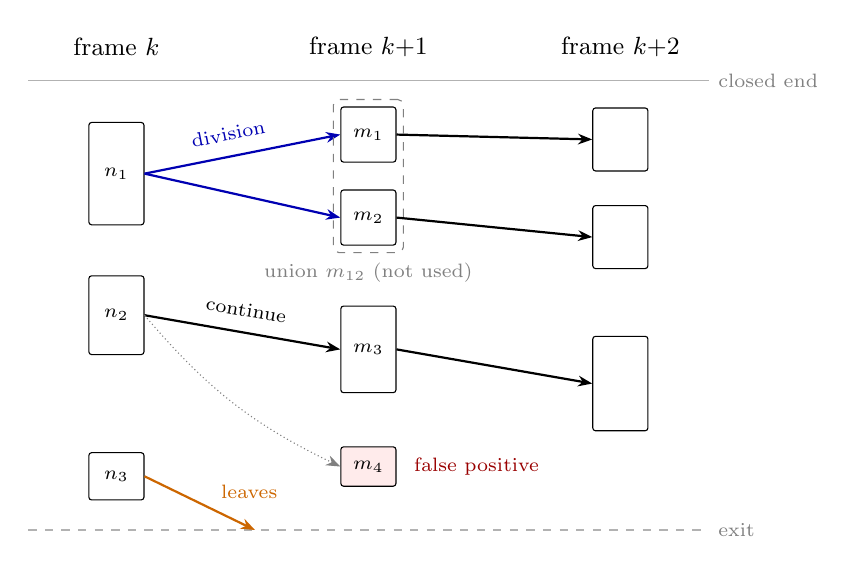
\begin{tikzpicture}[x=3.2cm,y=-0.62cm, >={Stealth[length=1.8mm]},
  nd/.style={draw, rounded corners=1pt, minimum width=7mm, inner sep=1pt, font=\scriptsize, fill=white},
  un/.style={nd, dashed, fill=gray!10, minimum width=5mm}]
\foreach \k/\lab in {0/{frame $k$},1/{frame $k{+}1$},2/{frame $k{+}2$}} \node[font=\small] at (\k,-1.2) {\lab};
\draw[gray!60] (-0.35,-0.5) -- (2.35,-0.5) node[right, font=\scriptsize, gray]{closed end};
\draw[gray!60, dashed] (-0.35,8.7) -- (2.35,8.7) node[right, font=\scriptsize, gray]{exit};
% frame k
\node[nd, minimum height=13mm] (A0) at (0,1.4) {$n_1$};
\node[nd, minimum height=10mm] (B0) at (0,4.3) {$n_2$};
\node[nd, minimum height=6mm]  (C0) at (0,7.6) {$n_3$};
% frame k+1
\node[nd, minimum height=7mm]  (A1) at (1,0.6) {$m_1$};
\node[nd, minimum height=7mm]  (A1b) at (1,2.3) {$m_2$};

\node[nd, minimum height=11mm] (B1) at (1,5.0) {$m_3$};
\node[nd, minimum height=5mm, fill=red!8]  (F1) at (1,7.4) {$m_4$};
% frame k+2
\node[nd, minimum height=8mm] (A2) at (2,0.7) {};
\node[nd, minimum height=8mm] (A2b) at (2,2.7) {};
\node[nd, minimum height=12mm] (B2) at (2,5.7) {};
% edges
\draw[->, thick, blue!70!black] (A0.east) -- node[pos=0.45, above=2pt, sloped, font=\scriptsize]{division} (A1.west);
\draw[->, thick, blue!70!black] (A0.east) -- (A1b.west);
\draw[->, thick] (B0.east) -- node[pos=0.5, above=2pt, sloped, font=\scriptsize]{continue} (B1.west);
\draw[->, thick, orange!80!black] (C0.east) -- node[pos=0.6, above right=0pt, font=\scriptsize]{leaves} (0.55,8.7);
\draw[->, thick] (A1.east) -- (A2.west);
\draw[->, thick] (A1b.east) -- (A2b.west);
\draw[->, thick] (B1.east) -- (B2.west);
\draw[->, gray, densely dotted] (B0.east) to[bend right=12] (F1.west);
\node[font=\scriptsize, red!60!black, right=1mm of F1] {false positive};
\node[draw, dashed, gray, rounded corners=2pt, inner sep=2.5pt, fit=(A1)(A1b), label={[font=\scriptsize, gray]below:union $m_{12}$ (not used)}] (U1) {};
\end{tikzpicture}
\caption{Candidate graph of three frames of a channel (top = closed end). Nodes are detections and unions of touching detections (dashed frame). Solid arrows: events of the chosen solution; dotted: a candidate event that was not chosen. The solution has $n_1$ dividing into $m_1,m_2$ (so the union $m_{12}$ is not used), $n_2$ continuing as $m_3$, $n_3$ leaving through the exit and $m_4$ declared a false positive. The constraints guarantee that every detection is explained exactly once and that the chosen links do not cross.}
\label{fig:graph}
\end{figure}

\paragraph{Variables.} All variables are binary (Fig.~\ref{fig:graph}):
\begin{itemize}
\item $z_n=1$ if node $n\in\mathcal N$ is a cell of the solution;
\item $f_j=1$ if detection $j$ is a false positive;
\item $u_n=1$ if a track starts at $n$ (appearance), $v_n=1$ if a track ends at $n$ (departure);
\item $x_e=1$ for a chosen continuation $e=(n\to m)\in\mathcal E_{\mathrm F}$;
\item $y_h=1$ for a chosen division $h=(n\to m_1,m_2)\in\mathcal E_{\mathrm D}$.
\end{itemize}
Write $\mathrm{in}(m)$ for the events whose target (or one of whose two targets) is $m$, and $\mathrm{out}(n)$ for the events whose source is $n$.

\paragraph{Objective.}
\begin{equation}
\min\;\sum_{n\in\mathcal N}\Bigl(\cost_{\mathrm{union}}\ind[n\text{ is a union}]\,z_n+\cost^{\mathrm{start}}_n u_n+\cost^{\mathrm{end}}_n v_n\Bigr)+\sum_{j}\cost_{\mathrm{fp}}c_j\,f_j+\sum_{e\in\mathcal E_{\mathrm F}}\cost_e\,x_e+\sum_{h\in\mathcal E_{\mathrm D}}\cost_h\,y_h.
\end{equation}

\paragraph{Constraints.}
\begin{align}
&\sum_{n:\;j\in\mathcal C(n)}z_n+f_j=1 && \forall j\in\textstyle\bigcup_k\mathcal D_k \qquad\text{(each detection explained once)}\label{eq:cover}\\
&z_m=u_m+\sum_{e\in\mathrm{in}(m)}x_e+\sum_{h\in\mathrm{in}(m)}y_h && \forall m\in\mathcal N\qquad\text{(one way in)}\label{eq:in}\\
&z_n=v_n+\sum_{e\in\mathrm{out}(n)}x_e+\sum_{h\in\mathrm{out}(n)}y_h && \forall n\in\mathcal N\qquad\text{(one way out)}\label{eq:out}\\
&x_e+x_{e'}\le1 && \forall\,(e,e')\text{ crossing}\qquad\text{(no overtaking)}\label{eq:cross}
\end{align}
Constraint~\eqref{eq:cover} says that a detection belongs either to exactly one chosen cell (by itself or inside a union) or is a false positive; in particular a union and its two parts cannot both be cells. Constraints~\eqref{eq:in}--\eqref{eq:out} say that every chosen cell has exactly one origin (it was there before, it is a daughter, or it appears) and exactly one fate (it continues, divides or leaves); a node that is not chosen ($z_n=0$) has no events. A division uses one unit of ``flow'' out of the mother and gives one unit to each daughter, which is why the problem is not a network flow and needs integer programming. Two links between the same pair of frames \emph{cross} if their order is inverted, $(a_n-a_{n'})(a_m-a_{m'})<0$; for divisions each daughter counts as a link. Constraint~\eqref{eq:cross} encodes the single-file geometry of the channel.

\paragraph{Lazy generation of the ordering constraints.} As in cutting-plane (row-generation) methods~\cite{dantzig1954}, the ordering constraints are added only when needed. The number of potentially crossing pairs is large, but very few of them are ever chosen. The ILP is therefore first solved without~\eqref{eq:cross}; the crossing pairs present in the solution are added as constraints, and the problem is solved again, until no crossing remains (at most 6 rounds per pass; typically 1--4). Because constraints are only added, each round can only increase the optimal cost, and the final solution is optimal for the full problem whenever it contains no crossing.

\paragraph{Solver.} The ILP is solved with HiGHS~\cite{huangfu2018} through \texttt{scipy.optimize.milp}~\cite{virtanen2020}, with a time limit of \SI{60}{\second} per segment. A channel has up to $\approx2\times10^4$ variables and is solved in about \SI{1}{\second} (up to \SI{20}{\second} for densely filled channels with 70 frames). If the solver fails, the channel is tracked with a frame-by-frame dynamic program (order-preserving assignment between consecutive frames with similar costs).

\subsection{Two passes}\label{sec:passes}
The first pass uses the position growth rate $\mu(t)$ for every cell. Each resulting track with at least three measured lengths not touching the exit gets its own rate, the least-squares slope of $\ln L$ against $t$,
\begin{equation}
\alpha_{\mathrm{track}}=\frac{\sum_i(t_i-\bar t)(\ln L_i-\overline{\ln L})}{\sum_i(t_i-\bar t)^2},\qquad\text{clipped to }[-0.02,\,0.06]\ \si{\per\minute},
\end{equation}
which is assigned to all its nodes and detections (and hence also enters the pushing term of the cells below). The ILP is then built and solved again. This lets slow-growing cells (e.g.\ old-pole mothers or antibiotic-treated cells) and fast-growing ones coexist in the same channel.

\subsection{From the solution to lineages}\label{sec:outputs}
Tracks are read off the solution: a track starts at a node with $u_n=1$ or at a daughter of a chosen division, and follows the chosen continuations until it ends ($v_n=1$) or divides. Each track is a cell with a unique number within the channel and a pointer to its mother. Its \emph{fate} is: division; exit (it was at, or would reach, the exit); disappearance inside the channel (death, lysis or loss); end of movie (seen in the last $1+g_{\max}$ frames of the segment); or lost before a long gap of bad frames.

\begin{itemize}
\item In frames where a tracked cell was not detected (gaps $g>0$) its box is linearly interpolated and flagged; it has no length. A cell first seen in frame 1 or 2 of a segment, or a daughter seen one frame after its sister, is back-filled into the missed frames if the space is free.
\item A length is not reported when the box touches the exit (truncated cell) or when its log-length deviates from the cell's own log-linear trend by more than $3\sigma_L$ (a detection that does not cover the whole cell).
\item Cells in channels cut by the image border are not measured.
\end{itemize}

\paragraph{Cell-cycle table.} For a cell born at $t_{\mathrm b}$ and dividing at $t_{\mathrm d}$ (a \emph{complete} cycle): the generation time $\tau=t_{\mathrm d}-t_{\mathrm b}$; the length at birth $L_0$ and at division $L_{\mathrm d}$, the first and last measured lengths (up to two frames from the event); the growth rate $\alpha$, the slope of $\ln L$ versus $t$ over all its measured frames (at least three); and the partition ratio $\pi=L_0/(L_0+L_0^{\mathrm{sister}})$; the birth is labelled symmetric if $0.3\le\pi\le0.7$, polar otherwise, and fragmentation if the mother produced three or more daughters. The tables are written as \texttt{<image>\_canales\_BF\_linaje.csv} (cell $\times$ frame) and \texttt{\_linaje\_ciclos.csv} (cell), and an RGB stack with one numbered box per cell is produced for visual inspection.

\begin{table}[ht]
\centering\small
\caption{Parameters of the global tracker (lengths in px, times in min).}
\label{tab:params}
\resizebox{\textwidth}{!}{%
\begin{tabular}{@{}llr@{}}
\toprule
Symbol & Meaning & Value\\
\midrule
$\sigma_0,\ \sigma_1$ & base position uncertainty; increase per px of predicted push & 3.0,\ 0.15\\
$\sigma_{\mathrm{free}},\ \sigma_{\mathrm{down}}$ & extra uncertainty for free chains; for moving below prediction & 5.0,\ 4.0\\
$\sigma_{\log L},\ \sigma_{\mathrm{px}}$ & relative and absolute length errors & 0.07,\ 2.0\\
$\tau_{\mathrm{pos}},\ \tau_{L}$ & caps of the position and length terms & 6,\ 12\\
$\kappa$ & touching distance (unions, chains) & 4\\
$\cost_{\mathrm{div}},\ \sigma_\pi,\ \cost_{\mathrm{young}}$ & division cost; partition scale; too-young penalty & 3,\ 0.12,\ 10\\
 & maximum gap between simultaneous daughters & 6\\
$\cost_{\mathrm{miss}}$ & per frame without detection & 3\\
$\cost_{\mathrm{new}},\ \cost_{\mathrm{init}}$ & appearance mid-movie; per frame from segment start & 16,\ 6\\
$\cost_{\mathrm{exit}},\ \cost_{\mathrm{disappear}}$ & leaving through the exit; disappearing inside & 0.5,\ 3\\
$H$ & horizon for ``would reach the exit'' (frames) & 4\\
$\cost_{\mathrm{fp}},\ \cost_{\mathrm{union}}$ & false positive ($\times$ confidence); union node & 12,\ 8\\
$g_{\max}$ & maximum number of missed frames in a continuation & 2\\
 & candidates per node (gap 0 / gap $>0$); maximum event cost & 6 / 2;\ 25\\
 & gates: down; up over other cells (per frame of gap) & 80;\ 25\\
 & collective shift: minimum, maximum, required improvement per cell & 4,\ 40,\ 4\\
 & default growth rate; track rate bounds (\si{\per\minute}) & 0.02;\ $[-0.02,0.06]$\\
 & new segment after a gap longer than & $\max(20, 3\overline{\Delta t})$\\
\bottomrule
\end{tabular}}
\end{table}

\subsection{Validation of the tracker}\label{sec:trk_eval}
\paragraph{Reference.} 46 channels with at least 30 consecutive manually annotated frames (5 conditions; \num{14916} annotated boxes) were linked into reference lineages by applying the frame-by-frame tracker to the manual boxes. Since these boxes are complete and correct, linking them is almost unambiguous; the reference lineages were inspected visually. A reference \emph{link} is either a continuation (the same cell in two consecutive frames) or a division (mother in frame $f$, daughter first seen in frame $f+1$): \num{14454} links in total, 850 of them divisions.

\paragraph{Metric.} In each frame the automatic cells are matched to the reference cells (Hungarian algorithm~\cite{kuhn1955} on IoU, threshold 0.5). A reference link $(f,A\to B)$ is reproduced if the automatic cells matched to $A$ in frame $f$ and to $B$ in frame $f+1$ are linked in the same way. This metric includes the errors of the detector (an undetected cell breaks its links). The automatic boxes cover \SI{98.6}{\percent} of the reference boxes.

\begin{table}[ht]
\centering\small
\caption{Fraction of reference links reproduced by the automatic lineage (installed detector). ``Global'': integer program of \S\ref{sec:ilp}; ``frame-by-frame'': order-preserving dynamic-programming assignment between consecutive frames with similar costs.}
\label{tab:trk}
\begin{tabular}{@{}lrrrcccc@{}}
\toprule
 & & \multicolumn{2}{c}{reference links} & \multicolumn{2}{c}{global} & \multicolumn{2}{c}{frame-by-frame}\\
\cmidrule(lr){3-4}\cmidrule(lr){5-6}\cmidrule(l){7-8}
Condition & channels & continue & divide & continue & divide & continue & divide\\
\midrule
LB & 5 & 3970 & 234 & 0.991 & 0.880 & 0.989 & 0.855\\
CIP \SI{0.1}{\micro\gram\per\milli\litre} & 5 & 1325 & 22 & 0.964 & 0.500 & 0.958 & 0.500\\
1\,h GEN 0.75 $\to$ CIP & 9 & 2612 & 162 & 0.951 & 0.802 & 0.945 & 0.809\\
2\,h GEN 0.75 $\to$ CIP & 5 & 1495 & 120 & 0.983 & 0.842 & 0.985 & 0.850\\
1\,h GEN 1.5 $\to$ CIP 0.02 & 22 & 4202 & 312 & 0.983 & 0.888 & 0.980 & 0.859\\
\midrule
All & 46 & 13604 & 850 & \textbf{0.977} & \textbf{0.853} & 0.975 & 0.838\\
\bottomrule
\end{tabular}
\end{table}

\paragraph{Results.} The global program reproduces \SI{97.7}{\percent} of the continuation links and \SI{85.3}{\percent} of the division links (Table~\ref{tab:trk}). Part of the remaining division disagreements are differences of one frame in the timing of the division (the network can resolve the septum before the annotator separates the two cells), which this metric counts as errors although the lineage is the same. The global formulation mainly helps where a frame-by-frame decision is ambiguous; with the earlier, less accurate detector the gain was larger (continuations \SI{96.0}{} $\to$ \SI{96.6}{\percent}, divisions \SI{72.5}{} $\to$ \SI{75.6}{\percent}), and the number of cells appearing without a mother in the middle of a movie dropped from 11--31 to 2--3 per position. The 46 channels were also used to train the detector, so these figures are somewhat optimistic for new images.

\paragraph{Biological plausibility without annotations.} In LB (positions 03--05 of 25/09) the automatic lineage contains 368, 412 and 426 complete cycles, of which \SI{93.5}{}, \SI{97.8}{} and \SI{94.8}{\percent} are plausible ($0.35\le\pi\le0.65$ and $1.4\le L_{\mathrm d}/L_0\le2.8$). This fraction was used as an annotation-free check when tuning the tracker.

%======================================================================
\section{Fluorescence quantification}\label{sec:fluo}
%======================================================================

When a position also carries a fluorescence channel (propidium iodide, or a GFP fusion such as NfsA--GFP), the fluorescence of every tracked cell is measured in every frame. The lineage itself is always built from bright field only (\S\S\ref{sec:detector}--\ref{sec:tracking}); fluorescence is read at the positions of the boxes found there.

\subsection{Images and geometry}
Each fluorescence image is paired with the bright-field image of the same position acquired within \SI{60}{\second} (\S\ref{sec:stacks}); with several fluorescence channels each one is measured separately and is shifted by the registration displacement of that bright-field slice, so both stacks share the same coordinates. Unlike bright field, fluorescence is kept at the camera's 16-bit depth, without any rescaling, so that intensities are comparable across frames, positions and days acquired with the same settings. Every channel is straightened with exactly the same geometry as in bright field (same axis, origin and width $W=\SI{33}{px}$), using bilinear interpolation. Let $S_t(r,w)$ denote the straightened fluorescence strip of a channel in frame $t$ (row $r$ along the channel, column $w=0,\dots,W-1$ across it).

\begin{figure}[ht]
\centering
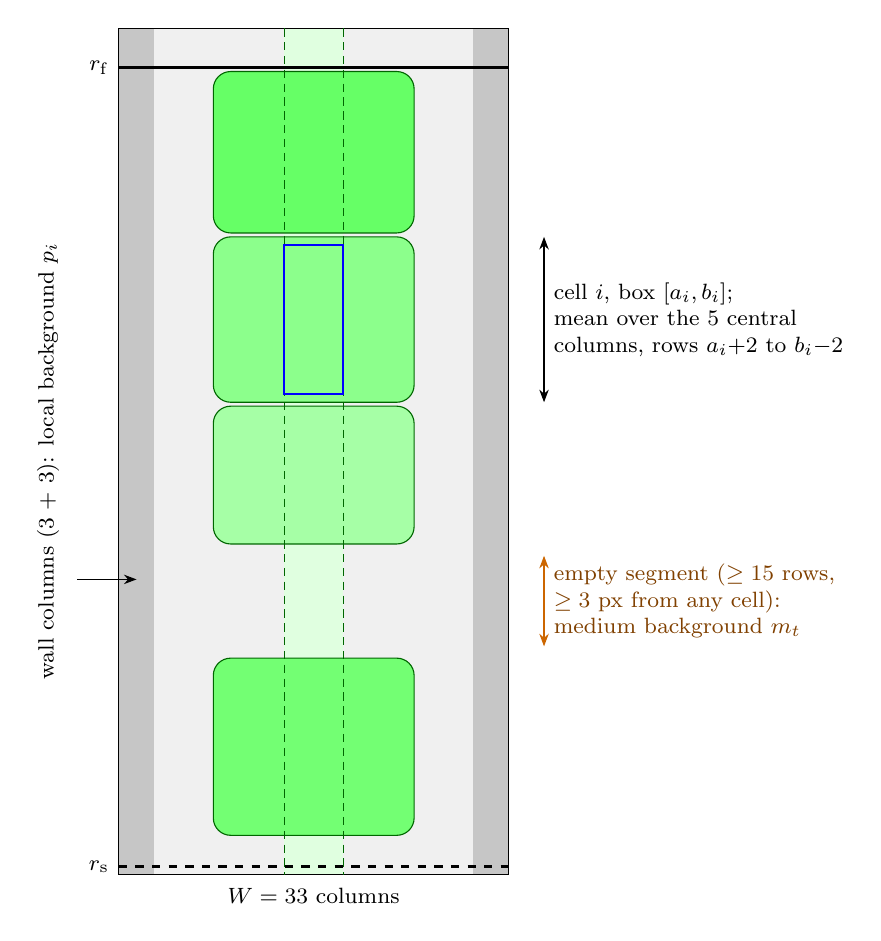
\begin{tikzpicture}[x=1.5mm,y=0.5mm,>={Stealth[length=1.6mm]},every node/.style={font=\footnotesize}]
  % strip: W = 33 columns, rows 0..215
  \fill[gray!12] (0,0) rectangle (33,-215);
  \fill[gray!45] (0,0) rectangle (3,-215);  \fill[gray!45] (30,0) rectangle (33,-215);
  \fill[green!12] (14,0) rectangle (19,-215);
  \draw (0,0) rectangle (33,-215);
  % closed end and exit
  \draw[very thick] (0,-10) -- (33,-10);  \node[left] at (0,-10) {$\rf$};
  \draw[very thick,dashed] (0,-213) -- (33,-213); \node[left] at (0,-213) {$\rs$};
  % cells (boxes [a,b])
  \foreach \a/\b/\s in {11/52/60, 53/95/45, 96/131/35, 160/205/55}{
     \fill[green!\s!black!0,fill=green!\s,rounded corners=2.2mm] (8,-\a) rectangle (25,-\b);
     \draw[green!40!black,rounded corners=2.2mm] (8,-\a) rectangle (25,-\b);}
  \draw[green!40!black,densely dashed] (14,0) -- (14,-215) (19,0) -- (19,-215);
  % measured interior of one cell (pole trim)
  \draw[thick,blue] (14,-55) rectangle (19,-93);
  \draw[<->] (36,-53) -- node[right,align=left] {cell $i$, box $[a_i,b_i]$;\\ mean over the 5 central\\ columns, rows $a_i{+}2$ to $b_i{-}2$} (36,-95);
  % empty segment
  \draw[<->,orange!80!black] (36,-134) -- node[right,align=left,text=orange!50!black] {empty segment ($\ge15$ rows,\\ $\ge3$ px from any cell):\\ medium background $m_t$} (36,-157);
  % walls
  \node[align=center,rotate=90] at (-6,-110) {wall columns (3 + 3): local background $p_i$};
  \draw[->] (-3.5,-140) -- (1.5,-140);
  \node[below,align=center] at (16.5,-216) {$W=33$ columns};
\end{tikzpicture}
\caption{Fluorescence measurement on a straightened channel (schematic, approximately to scale). Dashed lines: the five central columns, where the cell is in focus and widest. Dark grey: the three columns of PDMS wall on each side, used as the local background. Blue: the region averaged for one cell, i.e.\ its box without \SI{2}{px} at each pole. Orange: a stretch of channel without cells, used to estimate how much the medium itself fluoresces.}
\label{fig:fluo}
\end{figure}

\subsection{Raw signal and local background}
For a cell $i$ with box $[a_i,b_i]$ in frame $t$ (rows in the ImageJ convention of \S\ref{sec:channels}) the measured rows are
\begin{equation}
R_i=\bigl\{\,r\in\mathbb Z:\ \lfloor a_i+\tfrac12\rfloor+2\;\le r<\;\min\bigl(\lceil b_i+\tfrac12\rceil-2,\ \rs\bigr)\bigr\},
\end{equation}
that is, the box without \SI{2}{px} at each pole (the poles are blurred and partly mix with the neighbouring cell or with the dark gap between cells) and without the part outside the channel. Cells with $|R_i|<3$ are not measured. Let $C=\{14,\dots,18\}$ be the five central columns and $P=\{0,1,2\}\cup\{30,31,32\}$ the wall columns. The raw intensity and the local background of the cell are
\begin{equation}
\bar S_i=\frac{1}{|R_i|\,|C|}\sum_{r\in R_i}\sum_{w\in C}S_t(r,w),\qquad
p_i=\operatorname*{median}_{r\in R_i,\ w\in P}S_t(r,w).
\end{equation}
The wall background $p_i$ contains the camera offset, the autofluorescence of the PDMS and the out-of-focus light of the whole field. It is taken in the same rows and the same frame as the cell because it is not constant: it grows towards the exit of the channel (where the main trench and its cells are close) and drifts in time. The median, rather than the mean, makes it insensitive to a bright neighbouring cell that spills into the wall columns.

\subsection{Medium background}
The medium inside an empty channel is slightly brighter than the wall (it can contain fluorescent compounds, and the channel is a thin layer of liquid rather than PDMS). This offset is measured in the stretches of the channel where there are no cells. In frame $t$ a row $r$ of a channel is \emph{empty} if $\rf+3\le r<\rs-10$ and no box of that frame, enlarged by \SI{3}{px} at both ends, covers it. If a channel has a set $E$ of at least 15 empty rows, it contributes the value
\begin{equation}
\frac{1}{|E|\,|C|}\sum_{r\in E}\sum_{w\in C}S_t(r,w)\;-\;\operatorname*{median}_{r\in E,\ w\in P}S_t(r,w),
\end{equation}
and the medium background $m_t$ of the position in frame $t$ is the median of these values over all its channels; frames where no channel has an empty stretch get $m_t$ by linear interpolation in time.

\subsection{Concentration and amount}
The \emph{net fluorescence} of the cell is
\begin{equation}
c_i=\bar S_i-p_i-m_t .
\end{equation}
In wide-field imaging the light collected from a pixel is proportional to the number of fluorophores in the column of the cell below it. Because \emph{E.~coli} keeps an approximately constant width, the thickness of that column is the same in all cells, and $c_i$ is proportional to the \emph{concentration} of the fluorescent protein (arbitrary units). Multiplying by the length gives a quantity proportional to the total \emph{amount} of protein in the cell, $c_i\,L_i$ (with $L_i$ the length of \S\ref{sec:outputs}, or the box length when that is not available).

All visible cells are measured, but two kinds of measurement are flagged and excluded from the analyses: boxes that reach the exit (only the part inside the channel is measured; flag \texttt{toca\_salida}), and boxes interpolated in frames where the cell was not detected.
The table \texttt{<image>\_canales\_BF\_linaje\_<FLUO>.csv} has one row per cell and frame, with the raw mean $\bar S_i$, the backgrounds $p_i$ and $m_t$, the number of measured rows $|R_i|$, $c_i$ and $c_i L_i$.

For orientation, in the NfsA--GFP experiment of 16/10 (\num{98362} cell-frames) the median raw intensity was $\bar S=300$, the wall background $p=195$, the medium background $m=11$ and the net fluorescence $c=98$ (10--90th percentiles 37--209).

\subsection{Illumination correction}
The excitation light is not uniform over the field of view: in the 16/10 experiment the net fluorescence of channels on the right of the image was systematically higher than on the left, in every position and at every time. This is corrected by a smooth flat-field profile in the horizontal coordinate $x$ of the channel (the $x$ of its closed end in the image). Times are grouped into \SI{20}{\minute} bins; for each position $k$, bin $h$ and channel $j$, let $g_{khj}$ be the median net fluorescence of its cells (only cells with $c>5$, not interpolated and not at the exit), and keep the position-bins with at least 8 channels. A quadratic is fitted by least squares to all positions and times together,
\begin{equation}
\ln\frac{g_{khj}}{\operatorname*{median}_{j'}g_{khj'}}=\beta_0+\beta_1x_j+\beta_2x_j^2+\varepsilon_{khj},
\end{equation}
so that differences between conditions and times cancel out and only the dependence on the position in the field remains. The corrected concentration is $c_i/f(x_j)$, with $f(x)=\exp(\beta_1x+\beta_2x^2-\kappa)$ and $\kappa$ chosen so that $\ln f$ has mean zero across the field (the correction does not change the overall scale). In the 16/10 experiment $f$ varied by a factor $1.30$ from one side of the field to the other and explained \SI{5}{\percent} of the variance between channels. The profile is a property of the microscope and should be re-estimated for each experiment. This correction is applied in the analysis of the tables, not by \texttt{fluorescencia\_linaje.py}.

\subsection{Derived quantities}
\paragraph{Elongation rate.} Between consecutive frames of the same cell, $\mu=\Delta\ln L/\Delta t$ (\si{\per\minute}), using only measured lengths (not at the exit, not interpolated).

\paragraph{Production rate.} A change in concentration does not by itself mean a change in expression: a cell that stops growing accumulates protein even at a constant production, simply because it stops diluting it. If a cell of volume $V\propto L$ contains $N$ molecules and produces them at a rate $P$ (degradation of a stable GFP fusion being negligible on these time scales), then $c=N/V$ and
\begin{equation}
\frac{dc}{dt}=\frac{1}{V}\frac{dN}{dt}-\frac{N}{V^{2}}\frac{dV}{dt}=\frac{P}{V}-\mu c
\qquad\Longrightarrow\qquad
p\equiv\frac{P}{V}=\frac{dc}{dt}+\mu c ,
\end{equation}
where $\mu=\frac{1}{V}\frac{dV}{dt}=\frac{d\ln L}{dt}$. The production per unit volume $p$ is therefore estimated from finite differences of $c$ and from $\mu$; because it is a derivative it is noisy frame to frame and is computed on smoothed series (rolling medians of three frames, or population medians in \SI{10}{\minute} bins). At division $N$ and $V$ are both halved, so $c$ and $p$ are continuous along a line of cells (a cell and its upper daughter).

\paragraph{Measurement noise.} The concentration of a cell changes little between two frames \SIrange{3}{5}{\minute} apart, so the variation of $c$ between consecutive frames of the same cell estimates the measurement noise, $\mathrm{CV}_{\text{noise}}=\mathrm{sd}(c_{t+1}-c_t)/(\sqrt2\,\tilde c)$, with robust estimates of the spread (interquartile range$/1.349$) and of the centre (median $\tilde c$). In the 16/10 experiment it was \numrange{0.04}{0.08}, against a robust coefficient of variation between cells of about $0.20$; heterogeneity between cells is therefore well above measurement noise.

\paragraph{Caveats.} The fluorescence of a GFP fusion lags behind the protein by the maturation time of the fluorophore (minutes). The central-column mean is a concentration only if the cell fills the five columns, which holds for \emph{E.~coli} in these channels (it is several columns wider). Filaments that reach the exit are only partly measured, and neighbouring very bright cells can raise the signal near the poles, which is why the \SI{2}{px} at each pole are discarded.

%======================================================================
\section{Software}
%======================================================================
Python~3 with NumPy~\cite{harris2020}, SciPy~\cite{virtanen2020} (image filters, interpolation, \texttt{linear\_sum\_assignment}, \texttt{milp}/HiGHS~\cite{huangfu2018}), pandas~\cite{mckinney2010}, scikit-image~\cite{vanderwalt2014} (template matching, Otsu thresholds), scikit-learn~\cite{pedregosa2011} (fallback detector), tifffile~\cite{tifffile} and Matplotlib~\cite{hunter2007}; PyTorch~\cite{paszke2019} for training and ONNX Runtime~\cite{onnxruntime} for inference; Fiji~\cite{schindelin2012} for annotation and visual inspection. The whole pipeline (stacks $\to$ channels $\to$ detection and lineage $\to$ annotated stacks $\to$ mothers' sheet $\to$ fluorescence) is run from a single Jupyter~\cite{kluyver2016} notebook or step by step from the terminal; each step skips what is already up to date. Annotated stacks are written as losslessly compressed (deflate) TIFF files. The code, the trained models and their documentation are available at \url{https://github.com/jmolina07developer/mother-machine-pipeline} (GPL-3.0); they were written by Claude (Anthropic) working with J.~Molina, who designed the experiments, annotated the training data and validated the results.

%======================================================================
\section{Limitations}
%======================================================================
\begin{itemize}
\item Filaments longer than the channel are truncated at the exit; their length is not measured.
\item A cell that stops being detected inside the channel is classified as ``disappeared'': death, lysis and being flushed out cannot be distinguished from bright field alone.
\item The detector was trained on images acquired every 2--5 minutes; at \SI{15}{\minute} intervals and lower contrast (Ily) its recall drops (Table~\ref{tab:det}).
\item Division times can differ by one frame from manual annotation (the network detects the septum earlier).
\item Fluorescence is measured in arbitrary units; absolute comparisons between experiments require identical acquisition settings and a fresh illumination profile (\S\ref{sec:fluo}).
\end{itemize}

\begin{thebibliography}{99}
\bibitem{wang2010} P.~Wang, L.~Robert, J.~Pelletier, W.~L.~Dang, F.~Taddei, A.~Wright, S.~Jun. Robust growth of \emph{Escherichia coli}. \emph{Current Biology} 20:1099--1103 (2010).
\bibitem{schneider2012} C.~A.~Schneider, W.~S.~Rasband, K.~W.~Eliceiri. NIH Image to ImageJ: 25 years of image analysis. \emph{Nature Methods} 9:671--675 (2012).
\bibitem{otsu1979} N.~Otsu. A threshold selection method from gray-level histograms. \emph{IEEE Transactions on Systems, Man, and Cybernetics} 9:62--66 (1979).
\bibitem{liao2001} P.-S.~Liao, T.-S.~Chen, P.-C.~Chung. A fast algorithm for multilevel thresholding. \emph{Journal of Information Science and Engineering} 17:713--727 (2001).
\bibitem{reddy1996} B.~S.~Reddy, B.~N.~Chatterji. An FFT-based technique for translation, rotation, and scale-invariant image registration. \emph{IEEE Transactions on Image Processing} 5:1266--1271 (1996).
\bibitem{marr1980} D.~Marr, E.~Hildreth. Theory of edge detection. \emph{Proceedings of the Royal Society of London B} 207:187--217 (1980).
\bibitem{lewis1995} J.~P.~Lewis. Fast normalized cross-correlation. \emph{Vision Interface}, 120--123 (1995).
\bibitem{vanderwalt2014} S.~van~der~Walt, J.~L.~Sch\"onberger, J.~Nunez-Iglesias, F.~Boulogne, J.~D.~Warner, N.~Yager, E.~Gouillart, T.~Yu, and the scikit-image contributors. scikit-image: image processing in Python. \emph{PeerJ} 2:e453 (2014).
\bibitem{padfield2012} D.~Padfield. Masked object registration in the Fourier domain. \emph{IEEE Transactions on Image Processing} 21:2706--2718 (2012).
\bibitem{virtanen2020} P.~Virtanen, R.~Gommers, T.~E.~Oliphant, et al. SciPy~1.0: fundamental algorithms for scientific computing in Python. \emph{Nature Methods} 17:261--272 (2020).
\bibitem{zhou2019} X.~Zhou, D.~Wang, P.~Kr\"ahenb\"uhl. Objects as points. \emph{arXiv:1904.07850} (2019).
\bibitem{ronneberger2015} O.~Ronneberger, P.~Fischer, T.~Brox. U-Net: convolutional networks for biomedical image segmentation. \emph{MICCAI}, LNCS 9351, 234--241 (2015).
\bibitem{ioffe2015} S.~Ioffe, C.~Szegedy. Batch normalization: accelerating deep network training by reducing internal covariate shift. \emph{Proceedings of the 32nd International Conference on Machine Learning (ICML)}, PMLR 37:448--456 (2015).
\bibitem{nair2010} V.~Nair, G.~E.~Hinton. Rectified linear units improve restricted Boltzmann machines. \emph{Proceedings of the 27th International Conference on Machine Learning (ICML)}, 807--814 (2010).
\bibitem{yu2016} F.~Yu, V.~Koltun. Multi-scale context aggregation by dilated convolutions. \emph{International Conference on Learning Representations (ICLR)} (2016).
\bibitem{lin2017} T.-Y.~Lin, P.~Goyal, R.~Girshick, K.~He, P.~Doll\'ar. Focal loss for dense object detection. \emph{IEEE International Conference on Computer Vision (ICCV)}, 2980--2988 (2017).
\bibitem{schindelin2012} J.~Schindelin, I.~Arganda-Carreras, E.~Frise, et al. Fiji: an open-source platform for biological-image analysis. \emph{Nature Methods} 9:676--682 (2012).
\bibitem{paszke2019} A.~Paszke, S.~Gross, F.~Massa, A.~Lerer, J.~Bradbury, G.~Chanan, et al. PyTorch: an imperative style, high-performance deep learning library. \emph{Advances in Neural Information Processing Systems} 32, 8024--8035 (2019).
\bibitem{loshchilov2019} I.~Loshchilov, F.~Hutter. Decoupled weight decay regularization. \emph{International Conference on Learning Representations (ICLR)} (2019).
\bibitem{smith2019} L.~N.~Smith, N.~Topin. Super-convergence: very fast training of neural networks using large learning rates. \emph{Proc.\ SPIE} 11006, 1100612 (2019).
\bibitem{onnx} ONNX: Open Neural Network Exchange. \url{https://onnx.ai}.
\bibitem{onnxruntime} ONNX Runtime developers. ONNX Runtime. \url{https://onnxruntime.ai}.
\bibitem{kuhn1955} H.~W.~Kuhn. The Hungarian method for the assignment problem. \emph{Naval Research Logistics Quarterly} 2:83--97 (1955).
\bibitem{crouse2016} D.~F.~Crouse. On implementing 2D rectangular assignment algorithms. \emph{IEEE Transactions on Aerospace and Electronic Systems} 52:1679--1696 (2016).
\bibitem{friedman2001} J.~H.~Friedman. Greedy function approximation: a gradient boosting machine. \emph{Annals of Statistics} 29:1189--1232 (2001).
\bibitem{ke2017} G.~Ke, Q.~Meng, T.~Finley, T.~Wang, W.~Chen, W.~Ma, Q.~Ye, T.-Y.~Liu. LightGBM: a highly efficient gradient boosting decision tree. \emph{Advances in Neural Information Processing Systems} 30, 3146--3154 (2017).
\bibitem{pedregosa2011} F.~Pedregosa, G.~Varoquaux, A.~Gramfort, et al. Scikit-learn: machine learning in Python. \emph{Journal of Machine Learning Research} 12:2825--2830 (2011).
\bibitem{padfield2011} D.~Padfield, J.~Rittscher, B.~Roysam. Coupled minimum-cost flow cell tracking for high-throughput quantitative analysis. \emph{Medical Image Analysis} 15:650--668 (2011).
\bibitem{jug2014} F.~Jug, T.~Pietzsch, D.~Kainmueller, J.~Funke, M.~Kaiser, E.~van~Nimwegen, C.~Rother, G.~Myers. Optimal joint segmentation and tracking of \emph{Escherichia coli} in the mother machine. \emph{Bayesian and grAphical Models for Biomedical Imaging (BAMBI)}, LNCS 8677, 25--36 (2014).
\bibitem{schiegg2013} M.~Schiegg, P.~Hanslovsky, B.~X.~Kausler, L.~Hufnagel, F.~A.~Hamprecht. Conservation tracking. \emph{IEEE International Conference on Computer Vision (ICCV)}, 2928--2935 (2013).
\bibitem{dantzig1954} G.~Dantzig, R.~Fulkerson, S.~Johnson. Solution of a large-scale traveling-salesman problem. \emph{Journal of the Operations Research Society of America} 2:393--410 (1954).
\bibitem{huangfu2018} Q.~Huangfu, J.~A.~J.~Hall. Parallelizing the dual revised simplex method. \emph{Mathematical Programming Computation} 10:119--142 (2018).
\bibitem{harris2020} C.~R.~Harris, K.~J.~Millman, S.~J.~van~der~Walt, et al. Array programming with NumPy. \emph{Nature} 585:357--362 (2020).
\bibitem{mckinney2010} W.~McKinney. Data structures for statistical computing in Python. \emph{Proceedings of the 9th Python in Science Conference}, 56--61 (2010).
\bibitem{tifffile} C.~Gohlke. tifffile: read and write TIFF files. \url{https://github.com/cgohlke/tifffile}.
\bibitem{hunter2007} J.~D.~Hunter. Matplotlib: a 2D graphics environment. \emph{Computing in Science \& Engineering} 9:90--95 (2007).
\bibitem{kluyver2016} T.~Kluyver, B.~Ragan-Kelley, F.~P\'erez, et al. Jupyter Notebooks: a publishing format for reproducible computational workflows. In \emph{Positioning and Power in Academic Publishing: Players, Agents and Agendas}, IOS Press, 87--90 (2016).
\end{thebibliography}

\end{document}
